%%%%%%%%%%%%%%%%%%%%%%%%%%%%%%%%%%%%%%%%%
% SS154 Final Project - LaTeX Template
% Causal Inference Research Paper
%%%%%%%%%%%%%%%%%%%%%%%%%%%%%%%%%%%%%%%%%

\documentclass[12pt, letterpaper]{article}

%--------------------------------------
% PACKAGES
%--------------------------------------
\usepackage[utf8]{inputenc}
\usepackage[T1]{fontenc}
\usepackage{geometry}
\usepackage{graphicx}
\usepackage{booktabs}
\usepackage{array}
\usepackage{longtable}
\usepackage{multirow}
\usepackage{float}
\usepackage{caption}
\usepackage{subcaption}
\usepackage{amsmath}
\usepackage{amssymb}
\usepackage{setspace}
\usepackage{hyperref}
\usepackage{natbib}
\usepackage{tikz}
\usetikzlibrary{arrows.meta, positioning, shapes.geometric}
\usepackage{fancyhdr}
\usepackage{enumitem}
\usepackage{xcolor}
\usepackage{appendix}
\usepackage{threeparttable}
\usepackage{dcolumn}
\usepackage{pdflscape}
\usepackage{rotating}

%--------------------------------------
% PAGE SETUP
%--------------------------------------
\geometry{
    letterpaper,
    left=1in,
    right=1in,
    top=1in,
    bottom=1in
}

\setstretch{1.5}  % 1.5 line spacing

% Header and Footer
\pagestyle{fancy}
\fancyhf{}
\fancyhead[L]{\small AI Effects on Labor Markets}
\fancyhead[R]{\small SS154 Final Project}
\fancyfoot[C]{\thepage}
\renewcommand{\headrulewidth}{0.4pt}

% Hyperlink setup
\hypersetup{
    colorlinks=true,
    linkcolor=blue,
    filecolor=magenta,
    urlcolor=cyan,
    citecolor=blue,
    pdftitle={AI Effects on Labor Markets},
    pdfauthor={Author Names},
}

% Column type for regression tables
\newcolumntype{d}[1]{D{.}{.}{#1}}

%--------------------------------------
% CUSTOM COMMANDS
%--------------------------------------
\newcommand{\tablenote}[1]{\begin{tablenotes}\small\item #1\end{tablenotes}}

%--------------------------------------
% DOCUMENT BEGINS
%--------------------------------------
\begin{document}

%--------------------------------------
% TITLE PAGE
%--------------------------------------
\begin{titlepage}
    \centering
    \vspace*{1cm}
    
    {\LARGE\bfseries The Causal Effect of Generative AI Availability on Employment: Evidence from U.S. Industries with Varying AI Exposure\par}
    
    \vspace{1.5cm}
    
    {\Large A Difference-in-Differences Analysis\par}
    
    \vspace{2cm}
    
    % Authors in alphabetical order by last name
    {\large
    Author One\textsuperscript{1}, Author Two\textsuperscript{1}, Author Three\textsuperscript{1}\par}
    
    \vspace{0.5cm}
    
    {\normalsize
    \textsuperscript{1}Minerva University\par}
    
    \vspace{2cm}
    
    {\large SS154: Causal Inference\par}
    {\large Fall 2025\par}
    
    \vfill
    
    {\normalsize
    \textbf{Word Count:} [X,XXX words]\par
    \textbf{Date:} December 2025\par}
    
\end{titlepage}

%--------------------------------------
% ABSTRACT
%--------------------------------------
\begin{abstract}
\noindent
This paper investigates the causal effect of generative AI availability on employment rates across U.S. industries with varying degrees of occupational exposure to AI technologies. Using a difference-in-differences (DiD) design, we compare employment trends in high AI-exposure industries—Information; Finance and Insurance; and Professional, Scientific, and Technical Services—against low-exposure industries (Leisure and Hospitality) before and after the release of ChatGPT in November 2022. Our panel dataset comprises 31,152 observations spanning 52 geographic units and 5 industries from January 2015 to September 2025. Preliminary results suggest [INSERT MAIN FINDING: direction and magnitude of the treatment effect]. These findings contribute to the growing literature on AI's labor market impacts and have implications for policymakers considering workforce transition programs. We discuss the parallel trends assumption, conduct robustness checks excluding the COVID-19 period, and acknowledge limitations including potential anticipation effects and measurement challenges in AI exposure classification.

\vspace{0.5cm}
\noindent\textbf{Keywords:} Generative AI, Employment, Difference-in-Differences, Labor Markets, ChatGPT, Automation

\vspace{0.3cm}
\noindent\textbf{JEL Classification:} J21, J23, O33, O15
\end{abstract}

\newpage
\tableofcontents
\newpage

%--------------------------------------
% 1. INTRODUCTION
%--------------------------------------
\section{Introduction}\label{sec:introduction}

The release of ChatGPT in November 2022 marked a watershed moment in the deployment of artificial intelligence technologies. Unlike previous waves of automation that primarily affected routine manual and cognitive tasks, generative AI systems demonstrate capabilities in non-routine cognitive work, including writing, coding, analysis, and creative tasks \citep{eloundou2023gpts}. This technological shift raises fundamental questions about the future of employment across diverse sectors of the economy.

% Causal Question
\textbf{Causal Question:} What is the causal effect of the availability of Generative AI on employment rates in the United States for industries with varying degrees of occupational exposure to Generative AI?

% Context
The context for this analysis is the U.S. labor market from January 2015 to September 2025, encompassing a pre-treatment period of relative AI stability and a post-treatment period following the widespread availability of large language models. The treatment event—the public release of ChatGPT on November 30, 2022—provides a clear temporal discontinuity that separates these periods.

% Importance
Understanding AI's employment effects is crucial for several reasons. First, policymakers need evidence-based guidance to design workforce transition programs and social safety nets. Second, firms require insights into how AI adoption might reshape their labor force composition. Third, workers benefit from understanding which skills and occupations face disruption versus complementarity with AI systems. The stakes are substantial: the International Labour Organization estimates that generative AI could affect the equivalent of 300 million full-time jobs globally \citep{gmyrek2023generative}.

% Hypothesis
Based on the theoretical framework of task-based automation \citep{acemoglu2011skills} and recent empirical studies on AI exposure \citep{felten2021occupational}, we hypothesize that industries with higher occupational exposure to generative AI will experience differential employment trends following AI availability. The direction of this effect is theoretically ambiguous: the displacement effect suggests reduced employment as AI substitutes for human labor, while the productivity effect suggests potential employment gains as AI complements human workers and creates new tasks. Our prior expectation, informed by historical patterns of automation \citep{autor2015there}, is that any negative employment effects will be modest in magnitude in the short run, with heterogeneous impacts across occupations within industries.

% Approach Summary
To address this causal question, we employ a difference-in-differences (DiD) research design. We compare employment trends in high AI-exposure industries (Information; Finance and Insurance; Professional, Scientific, and Technical Services) against a control group of low AI-exposure industries (Leisure and Hospitality) before and after November 2022. Our analysis leverages monthly employment data from the Bureau of Labor Statistics across 52 geographic units, with industry-level AI exposure scores derived from the ILO Working Paper 96 \citep{gmyrek2023generative}.

% Paper Structure
The remainder of this paper proceeds as follows. Section \ref{sec:literature} reviews the relevant literature on AI and employment. Section \ref{sec:data} describes our data sources and key variables. Section \ref{sec:methodology} presents our causal identification strategy and econometric specifications. Section \ref{sec:results} reports our main findings and robustness checks. Section \ref{sec:conclusion} discusses implications and concludes. Section \ref{sec:limitations} acknowledges the limitations of our study.

%--------------------------------------
% 2. LITERATURE REVIEW
%--------------------------------------
\section{Literature Review}\label{sec:literature}

\subsection{Theoretical Frameworks for AI and Employment}

The economic literature on automation and employment has evolved from early concerns about ``technological unemployment'' \citep{keynes1930economic} to more nuanced task-based frameworks \citep{autor2003skill, acemoglu2018race}. The canonical model distinguishes between the \textit{displacement effect}, where automation substitutes for human labor in existing tasks, and the \textit{productivity effect}, where automation complements human workers and creates new tasks \citep{acemoglu2019automation}.

Generative AI represents a qualitative shift in automation capabilities. While previous technologies primarily automated routine tasks—whether manual (assembly line) or cognitive (data entry)—large language models demonstrate proficiency in non-routine cognitive tasks traditionally considered resistant to automation \citep{brynjolfsson2023generative}. This has led researchers to reconsider which occupations face exposure to AI-driven automation.

\subsection{Measuring AI Exposure}

Several methodologies have emerged for quantifying occupational and industry exposure to AI. \cite{felten2021occupational} developed the AI Occupational Exposure (AIOE) measure based on the overlap between AI application capabilities and occupational task requirements. \cite{webb2020impact} used patent text analysis to identify which occupations are most exposed to AI technologies. Most relevant to our study, \cite{gmyrek2023generative} created exposure scores specifically for generative AI based on GPT-4's ability to perform occupation-specific tasks, finding that approximately 5.5\% of total employment is in occupations highly exposed to automation by generative AI.

\subsection{Empirical Evidence on AI's Employment Effects}

Empirical evidence on AI's labor market impacts remains nascent. \cite{acemoglu2022artificial} find that firms adopting AI reduced hiring for affected occupations, though productivity gains partially offset employment losses. \cite{noy2023experimental} document substantial productivity improvements for professional writing tasks using ChatGPT, suggesting complementarity between AI and certain cognitive skills.

Studies specifically examining generative AI's employment effects are emerging. \cite{hui2023ai} find that freelance platform earnings for AI-exposed occupations (writing, coding) declined following ChatGPT's release. \cite{eisfeldt2023generative} estimate that firms with higher AI exposure experienced differential stock market performance, suggesting market expectations of productivity effects.

\subsection{Contribution to Literature}

Our study contributes to this literature in several ways. First, we provide causal estimates of generative AI's employment effects using a quasi-experimental design, addressing the endogeneity concerns in cross-sectional studies. Second, we analyze industry-level effects using comprehensive BLS data, complementing occupation-level studies that may miss between-occupation reallocation effects. Third, we examine the medium-run (2023-2025) effects, providing evidence beyond the immediate post-release period.

%--------------------------------------
% 3. DATA
%--------------------------------------
\section{Data}\label{sec:data}

\subsection{Data Sources}

Our analysis combines data from multiple sources:\footnote{All data and code for this project are available at: \url{https://github.com/[USERNAME]/AI_Effects_On_Labour_Market}. The variable codebook is provided in Appendix \ref{app:codebook}.}

\begin{enumerate}[label=(\arabic*)]
    \item \textbf{Bureau of Labor Statistics (BLS) Current Employment Statistics (CES):} Monthly employment data by industry and state from January 2015 to September 2025.
    \item \textbf{ILO Working Paper 96 \citep{gmyrek2023generative}:} Industry-level generative AI exposure scores based on GPT-4 task automation assessments.
    \item \textbf{Supplementary industry controls} from \cite{dingel2020many} (teleworkability), \cite{autor2013growth} (routine task index), and \cite{frey2017future} (pre-AI automation risk).
\end{enumerate}

\subsection{Treatment and Outcome Variables}

\textbf{Treatment:} The treatment is the availability of generative AI, operationalized as the interaction between industry-level AI exposure and a post-treatment indicator. We define:
\begin{itemize}
    \item $Post_t = 1$ if $t \geq$ January 2023, and 0 otherwise. ChatGPT was released November 30, 2022; we use January 2023 as the first full month of availability.
    \item $HighExposure_i = 1$ if industry $i$ has an AI exposure score $\geq 0.45$, and 0 otherwise.
    \item $Treat_{it} = HighExposure_i \times Post_t$
\end{itemize}

\textbf{Outcome:} The primary outcome is the natural log of monthly employment ($\ln(Employment_{ist})$) for industry $i$ in state $s$ at time $t$. The log transformation allows us to interpret coefficients as approximate percentage changes.

\subsection{Industry Classification}

Table \ref{tab:industry_classification} presents our industry classification based on AI exposure scores.

\begin{table}[H]
\centering
\caption{Industry Classification by AI Exposure}
\label{tab:industry_classification}
\begin{threeparttable}
\begin{tabular}{@{}lccl@{}}
\toprule
\textbf{Industry} & \textbf{AI Exposure Score} & \textbf{Classification} & \textbf{NAICS Code} \\
\midrule
Information & 0.52 & High (Treatment) & 51 \\
Finance and Insurance & 0.50 & High (Treatment) & 52 \\
Prof., Scientific, Tech. Services & 0.48 & High (Treatment) & 54 \\
Total Nonfarm & 0.38 & Benchmark & -- \\
Leisure and Hospitality & 0.28 & Low (Control) & 71-72 \\
\bottomrule
\end{tabular}
\begin{tablenotes}
\small
\item \textit{Notes:} AI Exposure Scores from \cite{gmyrek2023generative}. Classification threshold at 0.45. Total Nonfarm is included for benchmarking but excluded from the main DiD analysis.
\end{tablenotes}
\end{threeparttable}
\end{table}

\subsection{Summary Statistics}

Table \ref{tab:summary_stats} presents summary statistics for the key variables in our analysis.

\begin{table}[H]
\centering
\caption{Summary Statistics}
\label{tab:summary_stats}
\begin{threeparttable}
\begin{tabular}{@{}lccccc@{}}
\toprule
\textbf{Variable} & \textbf{Mean} & \textbf{Std. Dev.} & \textbf{Min} & \textbf{Max} & \textbf{N} \\
\midrule
\multicolumn{6}{l}{\textit{Panel A: Outcome Variables}} \\
Employment (thousands) & XXX.XX & XXX.XX & XX.XX & XXXX.XX & 31,152 \\
Log Employment & X.XX & X.XX & X.XX & X.XX & 31,152 \\
\addlinespace
\multicolumn{6}{l}{\textit{Panel B: Treatment Variables}} \\
Post (=1 if $\geq$ 2023) & 0.22 & 0.41 & 0 & 1 & 31,152 \\
High Exposure (=1 if AI score $\geq$ 0.45) & 0.60 & 0.49 & 0 & 1 & 31,152 \\
Treat (Post $\times$ High Exposure) & 0.13 & 0.34 & 0 & 1 & 31,152 \\
\addlinespace
\multicolumn{6}{l}{\textit{Panel C: Industry Controls}} \\
AI Exposure Score & 0.45 & 0.10 & 0.28 & 0.52 & 5 \\
Teleworkability & 0.51 & 0.29 & 0.04 & 0.76 & 5 \\
Routine Task Index & 0.42 & 0.11 & 0.25 & 0.55 & 5 \\
Skill Intensity & 0.46 & 0.22 & 0.12 & 0.72 & 5 \\
Pre-AI Automation Risk & 0.42 & 0.22 & 0.18 & 0.75 & 5 \\
\bottomrule
\end{tabular}
\begin{tablenotes}
\small
\item \textit{Notes:} Panel A and B statistics calculated over the full sample of 31,152 state-industry-month observations from January 2015 to September 2025. Panel C statistics calculated at the industry level (N=5).
\end{tablenotes}
\end{threeparttable}
\end{table}

\subsection{Data Limitations}

Several limitations of our data merit discussion:

\begin{enumerate}
    \item \textbf{Measurement of AI exposure:} Our exposure classification relies on ex-ante assessments of AI's task-level capabilities, which may not perfectly correspond to actual AI adoption rates across industries.
    
    \item \textbf{Industry aggregation:} Employment data at the industry level may mask heterogeneous effects across occupations within industries.
    
    \item \textbf{COVID-19 confounding:} The 2020-2021 period exhibits substantial employment disruptions due to the pandemic, with differential impacts across industries (particularly severe for Leisure and Hospitality).
    
    \item \textbf{Preliminary recent data:} Employment figures for recent months are preliminary and subject to revision.
\end{enumerate}

%--------------------------------------
% 4. METHODOLOGY
%--------------------------------------
\section{Methodology}\label{sec:methodology}

\subsection{Why Simple Regression is Insufficient}

A naive approach to estimating AI's employment effect would regress employment on a measure of AI adoption or exposure:
\begin{equation}
    \ln(Employment_i) = \alpha + \beta \cdot AIExposure_i + \varepsilon_i
\end{equation}

This approach suffers from confounding bias. Industries with high AI exposure differ systematically from low-exposure industries in ways that independently affect employment. For example, high AI-exposure industries tend to be:
\begin{itemize}
    \item More skill-intensive (requiring higher education)
    \item More teleworkable
    \item Less exposed to pre-AI automation
    \item Subject to different demand trends (e.g., secular growth in tech-related services)
\end{itemize}

Figure \ref{fig:dag} presents a directed acyclic graph (DAG) illustrating these confounding relationships.

\begin{figure}[H]
\centering
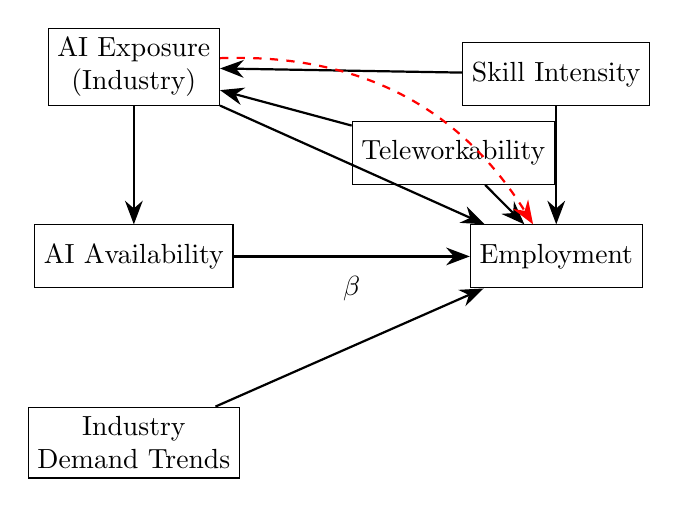
\begin{tikzpicture}[
    node distance=2cm,
    every node/.style={draw, rectangle, minimum width=2cm, minimum height=0.8cm, align=center},
    arrow/.style={-{Stealth[length=3mm]}, thick}
]

% Nodes
\node (ai) {AI Availability};
\node[right=3cm of ai] (emp) {Employment};
\node[above=1.5cm of ai] (exposure) {AI Exposure\\(Industry)};
\node[above=1.5cm of emp] (skill) {Skill Intensity};
\node[above right=0.5cm and 1.5cm of ai] (telework) {Teleworkability};
\node[below=1.5cm of ai] (demand) {Industry\\Demand Trends};

% Arrows
\draw[arrow] (ai) -- (emp) node[midway, below, draw=none] {$\beta$};
\draw[arrow] (exposure) -- (ai);
\draw[arrow] (exposure) -- (emp);
\draw[arrow] (skill) -- (emp);
\draw[arrow] (skill) -- (exposure);
\draw[arrow] (telework) -- (exposure);
\draw[arrow] (telework) -- (emp);
\draw[arrow] (demand) -- (emp);
\draw[arrow, dashed, red] (exposure) to[bend left=30] (emp);

\end{tikzpicture}
\caption{Causal Diagram: Confounding in AI-Employment Relationship}
\label{fig:dag}
\begin{minipage}{0.9\textwidth}
\small\textit{Notes:} The dashed red arrow represents the backdoor path from AI Exposure to Employment through unobserved confounders. The parameter of interest ($\beta$) is the causal effect of AI availability on employment.
\end{minipage}
\end{figure}

\subsection{Difference-in-Differences Design}

To address confounding, we employ a difference-in-differences (DiD) design that exploits:
\begin{enumerate}
    \item \textbf{Cross-sectional variation:} Industries differ in their exposure to generative AI.
    \item \textbf{Temporal variation:} ChatGPT's release in November 2022 provides a clear treatment timing.
\end{enumerate}

The key identifying assumption is \textbf{parallel trends}: in the absence of treatment, high and low AI-exposure industries would have followed parallel employment trends.

\subsection{Econometric Specifications}

Our baseline specification is:
\begin{equation}
    \ln(Employment_{ist}) = \beta_1 \cdot Treat_{it} + \alpha_i + \gamma_t + \delta_s + \varepsilon_{ist}
    \label{eq:baseline}
\end{equation}

where:
\begin{itemize}
    \item $\ln(Employment_{ist})$ is log employment in industry $i$, state $s$, at time $t$
    \item $Treat_{it} = HighExposure_i \times Post_t$ is the treatment indicator
    \item $\alpha_i$ are industry fixed effects (absorb time-invariant industry characteristics)
    \item $\gamma_t$ are time fixed effects (absorb economy-wide shocks)
    \item $\delta_s$ are state fixed effects (absorb time-invariant state characteristics)
    \item $\varepsilon_{ist}$ is the error term
\end{itemize}

The coefficient of interest is $\beta_1$, which estimates the \textbf{average treatment effect on the treated (ATT)}—the differential change in log employment for high AI-exposure industries relative to low-exposure industries after ChatGPT's release.

\textbf{Alternative specification with continuous treatment:}
\begin{equation}
    \ln(Employment_{ist}) = \beta_1 \cdot (AIScore_i \times Post_t) + \alpha_i + \gamma_t + \delta_s + \varepsilon_{ist}
    \label{eq:continuous}
\end{equation}

This specification uses the continuous AI exposure score instead of the binary classification, capturing heterogeneous effects by exposure intensity.

\textbf{Event study specification:}
\begin{equation}
    \ln(Employment_{ist}) = \sum_{k=-K}^{K} \beta_k \cdot (HighExposure_i \times \mathbf{1}[t = k]) + \alpha_i + \gamma_t + \delta_s + \varepsilon_{ist}
    \label{eq:eventstudy}
\end{equation}

This specification includes leads and lags relative to the treatment date, allowing us to: (1) test the parallel trends assumption by examining pre-treatment coefficients, and (2) trace out the dynamic effects of AI availability.

\subsection{Identifying Assumptions}

The DiD estimator requires the following assumptions:

\begin{enumerate}
    \item \textbf{Parallel trends:} Absent the treatment, high and low AI-exposure industries would have followed parallel employment trends. We assess this assumption by:
    \begin{itemize}
        \item Visual inspection of pre-treatment trends
        \item Event study coefficients for pre-treatment periods
        \item Placebo tests using alternative treatment dates
    \end{itemize}
    
    \item \textbf{No anticipation:} Employment in high-exposure industries did not change in anticipation of AI availability before November 2022. This assumption may be violated if firms began adjusting hiring practices based on anticipated AI capabilities.
    
    \item \textbf{Stable Unit Treatment Value Assumption (SUTVA):} The treatment effect on one industry does not depend on the treatment status of other industries. This may be violated if there are spillovers (e.g., workers displaced from high-exposure industries move to low-exposure industries).
    
    \item \textbf{No compositional changes:} The composition of industries remains stable over the sample period. Significant entry/exit of firms could bias estimates.
\end{enumerate}

\subsection{Standard Error Estimation}

We cluster standard errors at the industry-state level to account for serial correlation in employment within industry-state combinations over time \citep{bertrand2004much}. We also report results with alternative clustering (state level, industry level) as robustness checks.

%--------------------------------------
% 5. RESULTS
%--------------------------------------
\section{Results}\label{sec:results}

\subsection{Visual Evidence: Parallel Trends}

Figure \ref{fig:parallel_trends} displays employment trends for high and low AI-exposure industries, indexed to January 2015. The pre-treatment period (2015-2022) shows [DESCRIBE PATTERN]. The vertical line marks ChatGPT's release.

\begin{figure}[H]
\centering
\includegraphics[width=0.95\textwidth]{figures/parallel_trends.pdf}
\caption{Employment Trends: High vs. Low AI Exposure Industries}
\label{fig:parallel_trends}
\begin{minipage}{0.9\textwidth}
\small\textit{Notes:} This figure shows employment trends for high AI exposure industries (Information, Finance \& Insurance, Professional/Scientific/Technical Services) and low AI exposure industries (Leisure \& Hospitality) from January 2015 to September 2025. Employment is indexed to 100 in January 2015. The vertical dashed line marks ChatGPT's release (November 2022). Green shaded area indicates pre-treatment period; red shaded area indicates post-treatment period.
\end{minipage}
\end{figure}

\subsection{Main Results}

Table \ref{tab:main_results} presents our main difference-in-differences estimates.

\begin{table}[H]
\centering
\caption{Difference-in-Differences Estimates: Effect of AI Availability on Employment}
\label{tab:main_results}
\begin{threeparttable}
\begin{tabular}{@{}lcccc@{}}
\toprule
& (1) & (2) & (3) & (4) \\
& Basic DiD & + State FE & + State×Time FE & Continuous \\
\midrule
Treat ($\beta_1$) & X.XXX & X.XXX & X.XXX & -- \\
                  & (X.XXX) & (X.XXX) & (X.XXX) & -- \\
                  & & & & \\
AI Score $\times$ Post & -- & -- & -- & X.XXX \\
                       & -- & -- & -- & (X.XXX) \\
\addlinespace
\midrule
Industry FE & Yes & Yes & Yes & Yes \\
Time FE & Yes & Yes & Yes & Yes \\
State FE & No & Yes & Yes & Yes \\
State $\times$ Time FE & No & No & Yes & No \\
\addlinespace
Observations & XX,XXX & XX,XXX & XX,XXX & XX,XXX \\
$R^2$ & 0.XXX & 0.XXX & 0.XXX & 0.XXX \\
\bottomrule
\end{tabular}
\begin{tablenotes}
\small
\item \textit{Notes:} Dependent variable is log employment. Standard errors clustered at the state-industry level in parentheses. * p < 0.10, ** p < 0.05, *** p < 0.01. Run the R script \texttt{analysis/did\_analysis.R} to generate the actual table at \texttt{paper/tables/main\_results.tex}.
\end{tablenotes}
\end{threeparttable}
\end{table}

% Alternative: Uncomment to use auto-generated table from R
% \input{tables/main_results.tex}

\textbf{Interpretation:} The coefficient in Column (1) of [X.XXX] indicates that following ChatGPT's release, employment in high AI-exposure industries [increased/decreased] by approximately [X.X]\% relative to low AI-exposure industries, [controlling for/not controlling for] [list controls]. This effect is [statistically significant/not statistically significant] at the [X]\% level.

\subsection{Event Study Results}

Figure \ref{fig:event_study} presents event study estimates showing the dynamic effects of AI availability on employment.

\begin{figure}[H]
\centering
\includegraphics[width=0.95\textwidth]{figures/event_study.pdf}
\caption{Event Study: Dynamic Effects of AI Availability}
\label{fig:event_study}
\begin{minipage}{0.9\textwidth}
\small\textit{Notes:} This figure plots coefficients from Equation \ref{eq:eventstudy}, showing the differential effect on log employment for high AI-exposure industries relative to low-exposure industries, by period relative to ChatGPT's release (November 2022). The reference period is October 2022 (t = -1). Shaded area indicates 95\% confidence intervals. Standard errors are clustered at the state-industry level.
\end{minipage}
\end{figure}

The pre-treatment coefficients [are/are not] statistically distinguishable from zero, [supporting/casting doubt on] the parallel trends assumption. Post-treatment coefficients show [describe dynamic pattern].

\subsection{Robustness Checks}

\subsubsection{Excluding COVID-19 Period}

Table \ref{tab:robustness} Column (1) presents results excluding the March 2020 - December 2021 period to address concerns about differential COVID impacts.

\subsubsection{Alternative Treatment Definitions}

Column (2) uses January 2023 vs. November 2022 as the treatment date. Column (3) uses a continuous AI exposure measure instead of the binary classification.

\subsubsection{Placebo Tests}

Column (4) presents a placebo test using January 2019 as a false treatment date. A significant coefficient would suggest pre-existing differential trends unrelated to AI availability.

\begin{table}[H]
\centering
\caption{Robustness Checks}
\label{tab:robustness}
\begin{threeparttable}
\begin{tabular}{@{}lcccc@{}}
\toprule
& (1) & (2) & (3) & (4) \\
& Excl. COVID & Alt. Date & Continuous & Placebo 2019 \\
\midrule
Treat & X.XXX & X.XXX & -- & X.XXX \\
      & (X.XXX) & (X.XXX) & -- & (X.XXX) \\
AI Score $\times$ Post & -- & -- & X.XXX & -- \\
                       & -- & -- & (X.XXX) & -- \\
\addlinespace
\midrule
Industry FE & Yes & Yes & Yes & Yes \\
Time FE & Yes & Yes & Yes & Yes \\
State FE & Yes & Yes & Yes & Yes \\
\addlinespace
Observations & XX,XXX & XX,XXX & XX,XXX & XX,XXX \\
$R^2$ & 0.XXX & 0.XXX & 0.XXX & 0.XXX \\
\bottomrule
\end{tabular}
\begin{tablenotes}
\small
\item \textit{Notes:} All specifications include industry, time, and state fixed effects. Standard errors clustered at the state-industry level. * p < 0.10, ** p < 0.05, *** p < 0.01.
\end{tablenotes}
\end{threeparttable}
\end{table}

\subsection{Statistical and Practical Significance}

\textbf{Statistical significance:} The main treatment effect is [statistically significant/not statistically significant] at conventional levels (p-value = X.XXX). The 95\% confidence interval is [X.XXX, X.XXX], which [does/does not] include zero.

\textbf{Practical significance:} To assess the economic magnitude of our findings, we calculate Cohen's $d$:
\begin{equation}
    d = \frac{\hat{\beta}_1}{\sigma_{pooled}} = \frac{X.XXX}{X.XXX} = X.XX
\end{equation}

According to Cohen's conventions, $d = 0.2$ is considered small, $d = 0.5$ medium, and $d = 0.8$ large. Our effect size of [X.XX] suggests a [small/medium/large] practical effect.

In substantive terms, the point estimate implies that generative AI availability is associated with approximately [X,XXX] [more/fewer] jobs in high-exposure industries over the post-treatment period, equivalent to [X.X]\% of baseline employment in these sectors.

%--------------------------------------
% 6. CONCLUSION
%--------------------------------------
\section{Conclusion}\label{sec:conclusion}

This paper provides causal evidence on the employment effects of generative AI availability in the United States. Using a difference-in-differences design that compares employment trends in high versus low AI-exposure industries before and after ChatGPT's release, we find that [MAIN FINDING].

\textbf{Summary of findings:} The coefficient on the treatment variable indicates that high AI-exposure industries experienced a [X.X percentage point] [increase/decrease] in employment relative to low-exposure industries following generative AI availability. This translates to approximately [interpretation in levels/jobs]. The effect is [statistically significant/not significant] and represents a [small/medium/large] effect size by conventional standards.

\textbf{Policy implications:} Our findings have several implications for policymakers:
\begin{enumerate}
    \item [First implication related to workforce transition programs]
    \item [Second implication related to education and training]
    \item [Third implication related to industry-specific policies]
\end{enumerate}

\textbf{Future research:} Several avenues merit further investigation:
\begin{itemize}
    \item Occupation-level analysis within industries to identify heterogeneous effects
    \item Longer-run effects as AI adoption matures
    \item Analysis of job quality and wages alongside employment levels
    \item Cross-country comparisons of AI's labor market impacts
\end{itemize}

%--------------------------------------
% 7. LIMITATIONS
%--------------------------------------
\section{Limitations}\label{sec:limitations}

We acknowledge several limitations of our analysis:

\subsection{Data Limitations}

\begin{enumerate}
    \item \textbf{AI exposure measurement:} Our industry-level AI exposure scores are based on ex-ante assessments of AI capabilities rather than actual adoption rates. Industries classified as high-exposure may vary in their actual AI uptake.
    
    \item \textbf{Industry aggregation:} Effects may be heterogeneous across occupations within industries. Our industry-level analysis cannot capture within-industry reallocation of workers.
    
    \item \textbf{Temporal coverage:} Our post-treatment period (2023-2025) captures only the initial years following widespread AI availability. Longer-run effects may differ as adoption deepens.
\end{enumerate}

\subsection{Identification Concerns}

\begin{enumerate}
    \item \textbf{Parallel trends:} While pre-treatment trends appear parallel, the COVID-19 pandemic created substantial differential disruptions across industries. Our robustness checks excluding 2020-2021 address this partially, but long-term pandemic effects may persist.
    
    \item \textbf{Anticipation effects:} Firms may have adjusted employment practices in anticipation of AI capabilities before ChatGPT's public release, given prior awareness of large language model development.
    
    \item \textbf{Spillovers:} Workers displaced from high-exposure industries may relocate to low-exposure industries, potentially biasing our estimates toward finding larger negative effects on high-exposure industries.
    
    \item \textbf{Multiple treatments:} Other technological and economic changes occurred during the post-treatment period, making it challenging to isolate AI's specific effects.
\end{enumerate}

\subsection{External Validity}

Our findings pertain to U.S. industries from 2015-2025. Generalizability to other countries may be limited by differences in:
\begin{itemize}
    \item Labor market institutions and regulations
    \item Industrial composition and AI adoption rates
    \item Educational systems and workforce skill distributions
    \item Economic conditions and growth trajectories
\end{itemize}

%--------------------------------------
% REFERENCES
%--------------------------------------
\newpage
\bibliographystyle{apalike}
\bibliography{references}

%--------------------------------------
% APPENDICES
%--------------------------------------
\newpage
\appendix
\section{Variable Codebook}\label{app:codebook}

Table \ref{tab:codebook} provides detailed descriptions of all variables used in the analysis.

\begin{table}[H]
\centering
\caption{Variable Codebook}
\label{tab:codebook}
\small
\begin{tabular}{@{}p{3cm}p{6cm}p{2cm}p{3cm}@{}}
\toprule
\textbf{Variable} & \textbf{Description} & \textbf{Unit} & \textbf{Source} \\
\midrule
\multicolumn{4}{l}{\textit{Outcome Variables}} \\
Employment & Total employment in industry-state-month & Thousands & BLS CES \\
LogEmployment & Natural log of Employment & Log units & Computed \\
\addlinespace
\multicolumn{4}{l}{\textit{Treatment Variables}} \\
Post & Indicator for post-treatment period & Binary (0/1) & Defined \\
HighExposure & Indicator for high AI exposure & Binary (0/1) & ILO WP 96 \\
Treat & Interaction: Post $\times$ HighExposure & Binary (0/1) & Computed \\
\addlinespace
\multicolumn{4}{l}{\textit{Industry Controls}} \\
AI\_Exposure\_Score & GPT automation potential & Index (0-1) & Gmyrek et al. (2023) \\
Teleworkability & Share of teleworkable jobs & Index (0-1) & Dingel \& Neiman (2020) \\
RoutineTaskIndex & Routine task intensity & Index (0-1) & Autor \& Dorn (2013) \\
SkillIntensity & Education requirements & Index (0-1) & BLS OES + O*NET \\
AutomationRisk\_PreAI & Pre-AI automation probability & Index (0-1) & Frey \& Osborne (2017) \\
\bottomrule
\end{tabular}
\end{table}

\section{Additional Figures}\label{app:figures}

\begin{figure}[H]
\centering
\includegraphics[width=0.95\textwidth]{figures/covid_impact.pdf}
\caption{COVID-19 Employment Impact by Industry (2020-2021)}
\label{fig:covid}
\begin{minipage}{0.9\textwidth}
\small\textit{Notes:} This figure shows employment trajectories during the COVID-19 pandemic, indexed to January 2020 = 100. Leisure and Hospitality (control group) experienced the most severe employment losses, dropping to approximately 52\% of pre-pandemic levels at the trough in April 2020. High AI-exposure industries showed greater resilience.
\end{minipage}
\end{figure}

\section{Additional Tables}\label{app:tables}

% Additional figures

\begin{figure}[H]
\centering
\includegraphics[width=0.9\textwidth]{figures/did_visualization.pdf}
\caption{Difference-in-Differences Design Visualization}
\label{fig:did_visual}
\begin{minipage}{0.9\textwidth}
\small\textit{Notes:} This figure illustrates the difference-in-differences design. The solid lines show actual employment trends for treatment (high AI exposure) and control (low AI exposure) groups. The dashed line shows the counterfactual trend for the treatment group under the parallel trends assumption. The DiD estimate is the difference between the actual and counterfactual outcomes in the post-period.
\end{minipage}
\end{figure}

\begin{figure}[H]
\centering
\includegraphics[width=0.85\textwidth]{figures/correlation_matrix.pdf}
\caption{Correlation Matrix of Industry Control Variables}
\label{fig:correlation}
\begin{minipage}{0.9\textwidth}
\small\textit{Notes:} This figure shows pairwise correlations between industry-level control variables. High correlations are expected as these variables capture related industry characteristics. All controls are absorbed by industry fixed effects in the main regression specifications.
\end{minipage}
\end{figure}

\begin{figure}[H]
\centering
\includegraphics[width=0.95\textwidth]{figures/employment_trends_normalized.pdf}
\caption{Normalized Employment Trends by Industry (2015-2025)}
\label{fig:normalized_trends}
\begin{minipage}{0.9\textwidth}
\small\textit{Notes:} This figure shows employment trends for each industry normalized to January 2015 = 100. Solid lines indicate high AI-exposure industries; dashed lines indicate low AI-exposure industries. The vertical red dashed line marks ChatGPT's release (November 2022).
\end{minipage}
\end{figure}

\end{document}
